\documentclass[a4paper,12pt,twoside]{memoir}

% Castellano
\usepackage[spanish,es-tabla]{babel}
\selectlanguage{spanish}
\usepackage[utf8]{inputenc}
\usepackage[T1]{fontenc}
\usepackage{lmodern} % Scalable font
\usepackage{microtype}
\usepackage{placeins}
\usepackage{lipsum}
\RequirePackage{booktabs}
\RequirePackage[table]{xcolor}
\RequirePackage{xtab}
\RequirePackage{multirow}


\def\code#1{\texttt{#1}}

% Links
\PassOptionsToPackage{hyphens}{url}\usepackage[colorlinks]{hyperref}
\hypersetup{
	allcolors = {red}
}

% Ecuaciones
\usepackage{amsmath}

% Rutas de fichero / paquete
\newcommand{\ruta}[1]{{\sffamily #1}}

% Párrafos
\nonzeroparskip

% Huérfanas y viudas
\widowpenalty100000
\clubpenalty100000

% Imagenes
\usepackage{graphicx}
\newcommand{\imagen}[2]{
	\begin{figure}[!h]
		\centering
		\includegraphics[width=0.9\textwidth]{#1}
		\caption{#2}\label{fig:#1}
	\end{figure}
	\FloatBarrier
}

\newcommand{\imagenflotante}[2]{
	\begin{figure}%[!h]
		\centering
		\includegraphics[width=0.9\textwidth]{#1}
		\caption{#2}\label{fig:#1}
	\end{figure}
}



% El comando \figura nos permite insertar figuras comodamente, y utilizando
% siempre el mismo formato. Los parametros son:
% 1 -> Porcentaje del ancho de página que ocupará la figura (de 0 a 1)
% 2 --> Fichero de la imagen
% 3 --> Texto a pie de imagen
% 4 --> Etiqueta (label) para referencias
% 5 --> Opciones que queramos pasarle al \includegraphics
% 6 --> Opciones de posicionamiento a pasarle a \begin{figure}
\newcommand{\figuraConPosicion}[6]{%
  \setlength{\anchoFloat}{#1\textwidth}%
  \addtolength{\anchoFloat}{-4\fboxsep}%
  \setlength{\anchoFigura}{\anchoFloat}%
  \begin{figure}[#6]
    \begin{center}%
      \Ovalbox{%
        \begin{minipage}{\anchoFloat}%
          \begin{center}%
            \includegraphics[width=\anchoFigura,#5]{#2}%
            \caption{#3}%
            \label{#4}%
          \end{center}%
        \end{minipage}
      }%
    \end{center}%
  \end{figure}%
}

%
% Comando para incluir imágenes en formato apaisado (sin marco).
\newcommand{\figuraApaisadaSinMarco}[5]{%
  \begin{figure}%
    \begin{center}%
    \includegraphics[angle=90,height=#1\textheight,#5]{#2}%
    \caption{#3}%
    \label{#4}%
    \end{center}%
  \end{figure}%
}
% Para las tablas
\newcommand{\otoprule}{\midrule [\heavyrulewidth]}
%
% Nuevo comando para tablas pequeñas (menos de una página).
\newcommand{\tablaSmall}[5]{%
 \begin{table}
  \begin{center}
   \rowcolors {2}{gray!35}{}
   \begin{tabular}{#2}
    \toprule
    #4
    \otoprule
    #5
    \bottomrule
   \end{tabular}
   \caption{#1}
   \label{tabla:#3}
  \end{center}
 \end{table}
}

%
% Nuevo comando para tablas pequeñas (menos de una página).
\newcommand{\tablaSmallSinColores}[5]{%
 \begin{table}[H]
  \begin{center}
   \begin{tabular}{#2}
    \toprule
    #4
    \otoprule
    #5
    \bottomrule
   \end{tabular}
   \caption{#1}
   \label{tabla:#3}
  \end{center}
 \end{table}
}

\newcommand{\tablaApaisadaSmall}[5]{%
\begin{landscape}
  \begin{table}
   \begin{center}
    \rowcolors {2}{gray!35}{}
    \begin{tabular}{#2}
     \toprule
     #4
     \otoprule
     #5
     \bottomrule
    \end{tabular}
    \caption{#1}
    \label{tabla:#3}
   \end{center}
  \end{table}
\end{landscape}
}

%
% Nuevo comando para tablas grandes con cabecera y filas alternas coloreadas en gris.
\newcommand{\tabla}[6]{%
  \begin{center}
    \tablefirsthead{
      \toprule
      #5
      \otoprule
    }
    \tablehead{
      \multicolumn{#3}{l}{\small\sl continúa desde la página anterior}\\
      \toprule
      #5
      \otoprule
    }
    \tabletail{
      \hline
      \multicolumn{#3}{r}{\small\sl continúa en la página siguiente}\\
    }
    \tablelasttail{
      \hline
    }
    \bottomcaption{#1}
    \rowcolors {2}{gray!35}{}
    \begin{xtabular}{#2}
      #6
      \bottomrule
    \end{xtabular}
    \label{tabla:#4}
  \end{center}
}

%
% Nuevo comando para tablas grandes con cabecera.
\newcommand{\tablaSinColores}[6]{%
  \begin{center}
    \tablefirsthead{
      \toprule
      #5
      \otoprule
    }
    \tablehead{
      \multicolumn{#3}{l}{\small\sl continúa desde la página anterior}\\
      \toprule
      #5
      \otoprule
    }
    \tabletail{
      \hline
      \multicolumn{#3}{r}{\small\sl continúa en la página siguiente}\\
    }
    \tablelasttail{
      \hline
    }
    \bottomcaption{#1}
    \begin{xtabular}{#2}
      #6
      \bottomrule
    \end{xtabular}
    \label{tabla:#4}
  \end{center}
}

%
% Nuevo comando para tablas grandes sin cabecera.
\newcommand{\tablaSinCabecera}[5]{%
  \begin{center}
    \tablefirsthead{
      \toprule
    }
    \tablehead{
      \multicolumn{#3}{l}{\small\sl continúa desde la página anterior}\\
      \hline
    }
    \tabletail{
      \hline
      \multicolumn{#3}{r}{\small\sl continúa en la página siguiente}\\
    }
    \tablelasttail{
      \hline
    }
    \bottomcaption{#1}
  \begin{xtabular}{#2}
    #5
   \bottomrule
  \end{xtabular}
  \label{tabla:#4}
  \end{center}
}



\definecolor{cgoLight}{HTML}{EEEEEE}
\definecolor{cgoExtralight}{HTML}{FFFFFF}

%
% Nuevo comando para tablas grandes sin cabecera.
\newcommand{\tablaSinCabeceraConBandas}[5]{%
  \begin{center}
    \tablefirsthead{
      \toprule
    }
    \tablehead{
      \multicolumn{#3}{l}{\small\sl continúa desde la página anterior}\\
      \hline
    }
    \tabletail{
      \hline
      \multicolumn{#3}{r}{\small\sl continúa en la página siguiente}\\
    }
    \tablelasttail{
      \hline
    }
    \bottomcaption{#1}
    \rowcolors[]{1}{cgoExtralight}{cgoLight}

  \begin{xtabular}{#2}
    #5
   \bottomrule
  \end{xtabular}
  \label{tabla:#4}
  \end{center}
}



\graphicspath{ {./img/} }

% Capítulos
\chapterstyle{bianchi}
\newcommand{\capitulo}[2]{
	\setcounter{chapter}{#1}
	\setcounter{section}{0}
	\setcounter{figure}{0}
	\setcounter{table}{0}
	\chapter*{#2}
	\addcontentsline{toc}{chapter}{#2}
	\markboth{#2}{#2}
}

% Apéndices
\renewcommand{\appendixname}{Apéndice}
\renewcommand*\cftappendixname{\appendixname}

\newcommand{\apendice}[1]{
	%\renewcommand{\thechapter}{A}
	\chapter{#1}
}

\renewcommand*\cftappendixname{\appendixname\ }

% Formato de portada
\makeatletter
\usepackage{xcolor}
\newcommand{\tutor}[1]{\def\@tutor{#1}}
\newcommand{\course}[1]{\def\@course{#1}}
\definecolor{cpardoBox}{HTML}{E6E6FF}
\def\maketitle{
  \null
  \thispagestyle{empty}
  % Cabecera ----------------
\noindent
\includegraphics[width=\textwidth]{cabecera}\vspace{1cm}%
  \vfill
  % Título proyecto y escudo informática ----------------
  \colorbox{cpardoBox}{%
    \begin{minipage}{.8\textwidth}
      \vspace{.5cm}\Large
      \begin{center}
      \textbf{TFG del Grado en Ingeniería Informática}\vspace{.6cm}\\
      \textbf{\LARGE\@title{}}\\\\
      \vspace{.3cm}
      \large{Sistema de Gestión, Análisis y Recomendación de Biblioteca Musical de Spotify apoyado por Inteligencia Artificial}\\
      \vspace{.2cm}
      \small{\href{https://spotmyfm.jorgeruizdev.com}{spotmyfm.jorgeruizdev.com}}
      \end{center}
      \vspace{.2cm}
    \end{minipage}

  }%
  \hfill\begin{minipage}{.20\textwidth}
    
\includegraphics[width=\textwidth]{escudoInfor}
  \end{minipage}
  
  
  \vfill
  % Datos de alumno, curso y tutores ------------------
  
  \begin{center}%
  {%
    \noindent\LARGE
    Presentado por \@author{}\\ 
    en Universidad de Burgos --- \@date{}\\
    Tutor: \@tutor{}\\
  }%
  \end{center}%
  \null
  \cleardoublepage
  }
\makeatother

\newcommand{\nombre}{Jorge Ruiz Gómez} %%% cambio de comando

% Datos de portada
\title{SpotMyFM}
\author{\nombre}

\tutor{Bruno Baruque Zanón}
\date{\today}

\begin{document}

\maketitle


\newpage\null\thispagestyle{empty}\newpage


%%%%%%%%%%%%%%%%%%%%%%%%%%%%%%%%%%%%%%%%%%%%%%%%%%%%%%%%%%%%%%%%%%%%%%%%%%%%%%%%%%%%%%%%
\thispagestyle{empty}


\noindent
\includegraphics[width=\textwidth]{cabecera}\vspace{1cm}

\noindent D. Bruno Baruque Zanón, profesor del departamento de Ingeniería Informática, área de Ciencia de la Computación e Ingeligencia Artificial.

\noindent Expone:

\noindent Que el alumno D. \nombre, con DNI ---, ha realizado el Trabajo final de Grado en Ingeniería Informática titulado SpotMyFM. 

\noindent Y que dicho trabajo ha sido realizado por el alumno bajo la dirección del que suscribe, en virtud de lo cual se autoriza su presentación y defensa.

\begin{center} %\large
En Burgos, {\large \today}
\end{center}

\vfill\vfill\vfill

% Author and supervisor
\begin{minipage}{0.45\textwidth}
\begin{flushleft} %\large
Vº. Bº. del Tutor:\\[2cm]
D. Bruno Baruque Zanón
\end{flushleft}
\end{minipage}
\hfill
\hfill

\vfill

% para casos con solo un tutor comentar lo anterior
% y descomentar lo siguiente
%Vº. Bº. del Tutor:\\[2cm]
%D. nombre tutor


\newpage\null\thispagestyle{empty}\newpage




\frontmatter

% Abstract en castellano
\renewcommand*\abstractname{Resumen}
\begin{abstract}
Spotify es una de las plataformas de música en streaming más importantes del mundo. Se propone aumentar las funcionalidades de Spotify a partir de su API pública y otros servicios. 

Se plantea el desarrollo y despliegue de una plataforma web que permita a los usuarios de Spotify explorar y gestionar su biblioteca de una manera más avanzada y transparente a la que ofrece Spotify por defecto. 

La plataforma estará acompañada por una base de datos y un servicio de recuperación de información musical\footnote{Campo de investigación dedicado al análisis, modificación y creación de música a partir de diversas técnicas.}, que extraerá características de la señal de sonido de la canción y permitirá asociar géneros, subgéneros y estados de ánimo musicales a las distintas pistas; se utilizarán tres fuentes de datos, la API pública de Spotify, la API pública de LastFM y la API de SpotMyFM.

\end{abstract}

\renewcommand*\abstractname{Descriptores}
\begin{abstract}
Recuperación de información musical, CNN, Spotify, plataforma web, sistema de recomendación musical\footnote{Sistema que permite predecir la preferencia de usuario ante una serie de canciones.}.
\end{abstract}

\clearpage

% Abstract en inglés
\renewcommand*\abstractname{Abstract}
\begin{abstract}
Globally, Spotify is one of the most important music streaming platforms. This project aims to improve Spotify's functionalities based on its public API and other services.

This project explores the development and deployment of a web platform that allows Spotify users to explore and manage their library in a more advanced and transparent way than the one offered by Spotify.

The platform will be supported by a database and a music information retrieval service (MIR), which will extract features from the sound signal of the song and associate genres, subgenres, and musical moods to the different tracks; three data sources will be used, Spotify's public API, LastFM's public API, and SpotMyFM API.

\end{abstract}

\renewcommand*\abstractname{Keywords}
\begin{abstract}
Music information retrieval, CNN, Spotify, web platform, recommender system.
\end{abstract}

\clearpage

% Indices
\tableofcontents

\clearpage

\listoffigures

\clearpage

\listoftables
\clearpage

\mainmatter
\capitulo{1}{Introducción}

Descripción del contenido del trabajo y del estrucutra de la memoria y del resto de materiales entregados.

\capitulo{2}{Objetivos del proyecto}

Este apartado explica de forma precisa y concisa cuales son los objetivos que se persiguen con la realización del proyecto. Se puede distinguir entre los objetivos marcados por los requisitos del software a construir y los objetivos de carácter técnico que plantea a la hora de llevar a la práctica el proyecto.

\capitulo{3}{Conceptos Teóricos}

Una de las funcionalidades planteadas para la plataforma es etiquetar automáticamente los géneros, subgéneros y estados de ánimo de canciones a partir de su onda sonora. Para ello se han utilizado técnicas de aprendizaje aprendizaje profundo, ya que según el artículo \cite{deeplearn_vs_trad} presentan un mejor resultado que las técnicas de aprendizaje automático tradicionales.\footnote{KNN, SVM, Random Forest, MLP y Regresión Logística.}


\section{Conceptos Sonido}
\subsection{Onda Digital y Frecuencia de Muestreo}
Una onda analógica es una señal continua a lo largo del tiempo. Para poder trabajar con una onda digitalmente, es necesario discretizar la señal analógica en una señal digital.
Para ello, se declara una frecuencia de muestreo que indica cada cuantas medidas discretas se realizan sobre la amplitud de la onda en una señal analógica a lo largo del tiempo. En nuestro caso vamos a trabajar con una frecuencia de muestreo de $22050 Hz$, es decir, se van a tomar $22050$ puntos discretos de la amplitud de una onda cada segundo.\\
Este proceso de discretización de una señal digital es conocido como \textbf{modulación por impulsos codificados}. El formato de audio .wav almacena el audio sin comprimir directamente con esta modulación, por eso será utilizado a lo largo del proyecto en vez de otros formatos con mejor compresión como .mp3.


\subsection{Coeficientes Cepstrales en las Frecuencias de
Mel}\label{coeficientes-cepstrales-en-las-frecuencias-de-mel}


\begin{figure}
    \centering
    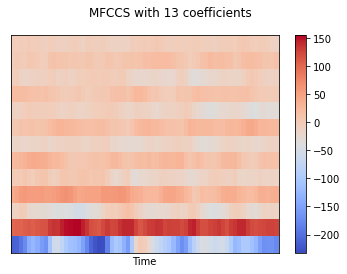
\includegraphics{img/3/mfcc.png}
    \caption{MFCC de un fragmento de 30s de una canción. Extraído de spotmyfm/Ludwig/notebooks/gtzan/mfcc.ipynb}
    \label{fig:MFCC}
\end{figure}
Los coeficientes cepstrales en las frecuencias de mel o MFCC Fig.\ref{fig:MFCC} son un tipo
de representación de la densidad espectral del sonido que intentan
representar la percepción auditiva humana.

Son muy utilizados en tareas de reconocimiento del habla y recuperación
de información musical.

Estos coeficientes están ajustados sobre la \textbf{escala de mel}, una
escala que aproxima la escala de tono a una escala similar a la
percepción humana, mejorando la representación del sonido.

Para obtener los MFCC partimos del espectrograma de mel, un
espectrograma ajustado a la escala de mel. En este caso, estamos
intentando obtener el espectrograma de un espectrograma, también conocido como cepstrum.

Un método para calcular los MFCCs puede\footnote{Cada biblioteca tiene una aproximación diferente.} ser el siguiente:

\begin{enumerate}
\def\labelenumi{\arabic{enumi}.}
\item
  Separar la señal en segmentos (hop\_length)
\item
  Aplicar la Transformada Discreta de Fourier a cada segmento para
  obtener la \textbf{potencia espectral}.
\item
  Transformar los resultados del paso 2 a la escala de mel.
\item
  Aplicar el logaritmo a cada frecuencia de mel, (escala logarítmica en
  \textbf{decibelios}).
\item
  Aplicar la Transformada Discreta del Coseno al resultado del paso 4
\item
  Escoger $N$ MFFCs\footnote{En \ref{fig:MFCC} se han escogido $N=13$ MFCCs}.
\end{enumerate}

Los pasos 1-3 se corresponden con la obtención de un espectrograma de mel.

Se recomienda consultar el apéndice A de \cite{book_mfcc} para consultar los detalles de la extracción. 

\section{Clasificación mediante Redes Neuronales
Convolucionales}\label{clasificacion_cnn}

Las redes neuronales convolucionales son una de las arquitecturas
neuronales más utilizadas en visión artificial debido a su poder para detectar patrones en imágenes, en nuestro caso vamos a buscar patrones en una representación bidimensional del sonido, los MFCCs \ref{coeficientes-cepstrales-en-las-frecuencias-de-mel}. Estas redes suelen estar formadas por una serie de bloques
convolucionales, seguidos de una o varias capas densas en la salida de
la red, como muestra \ref{fig:bloque_conv}.
La zona aizquierda de la línea discontinua roja compone la parte convolucional de la red, mientras que a la derecha de la línea se encuentra la parte densa de la red. Las última capa densa, compuesta por 3 neuronas, hace referencia a la capa de salida. 

\begin{figure}[h]
\centering
\label{fig:bloque_conv}
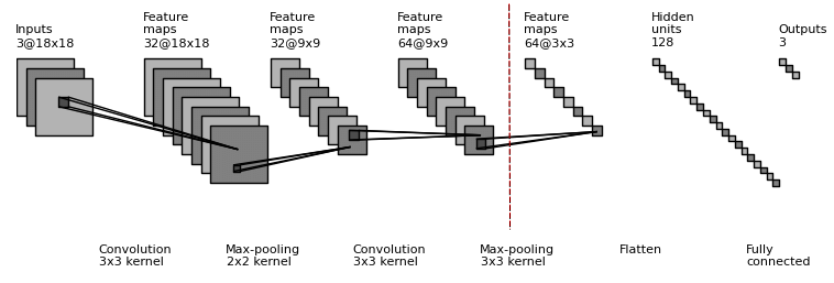
\includegraphics[width=2.99679in,height=1.01667in]{img/memoria/3/cnn.png}
\caption{Arquitectura de una red convolucional. Extraído de \cite{CNN_architecture} }
\end{figure}
\hypertarget{bloque-convolucional}{%
\subsection{Bloque Convolucional}\label{bloque-convolucional}}

Estos bloques, formados por capas, buscan resaltar los elementos más
relevantes en los datos a partir de las
operaciones de convolución y pooling.

La operación de convolución está formada por un kernel o filtro Fig.\ref{fig:kernel} que se
aplica Fig.\ref{fig:cnn_operation} a través de los datos. En el caso de la capa de convolución, los
pesos entrenables de dicha capa son el propio kernel.

\begin{figure}
    \centering
    \label{fig:kernel}
    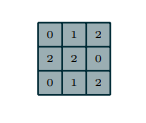
\includegraphics{img/memoria/3/kernel.png}
    \caption{Kernel 3x3. Extraído de \cite{convolution_guide}}
\end{figure}

Esta operación puede estar acompañada por una función de activación para
cada una de las neuronas, como por el ejemplo la función de activación
RELU \eqref{eq:relu_cnn}.

\begin{equation}
    \label{eq:relu_cnn}
    Relu(x) = max(0,x)
\end{equation}

\begin{figure}
    \centering
    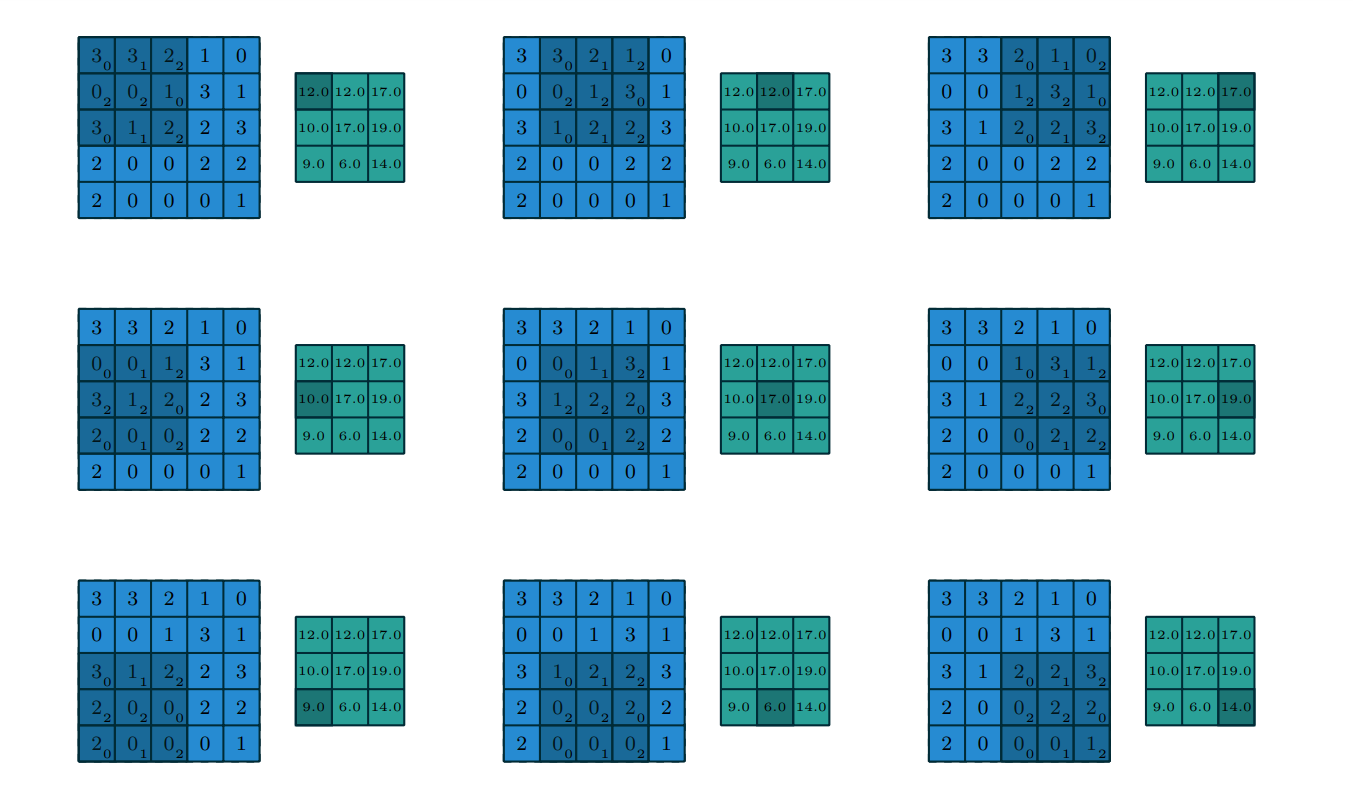
\includegraphics[width=5.90556in,height=3.52639in]{img/memoria/3/convolution.png}
    \caption{Aplicación del kernel 3x3 sobre un área 5x5. Extraído de \cite{convolution_guide}}
    \label{fig:cnn_operation}
\end{figure}

Por otro lado, la operación de pooling intenta reducir el tamaño de la
entrada, dejando solo los datos relevantes de un área. Se aplica de la
misma manera que una convolución, pero en vez de aplicar un kernel,
realizamos una operación aritmética sobre el área, como obtener el valor
más grande del área (Max Pooling) o la media de todos los valores
(Average Pooling)

Un bloque convolucional puede contener otras capas, como capas de
normalización, que normalizan de nuevo los datos para trabajar siempre
en el intervalo {[}0,1{]} o [-1, 1].

\hypertarget{densa}{%
\subsection{Densa}\label{densa}}

La salida de una red neuronal puede estar formada por capas densas, estas capas
tienen una entrada unidimensional, por lo que si la salida del último
bloque convolucional no es unidimensional, es necesario utilizar una
operación de Flatten que transforma la matriz de entrada en una única
fila concatenando cada una de las filas de la matriz.\\
En este tipo de arquitectura, cada una de las neuronas de una capa se interconectan con todas las neuronas de la capa siguiente. 

Cada neurona está formada por:

\begin{itemize}
\item
  Entradas ($[x_1 \dots x_n]$)
\item
  Salida  ($y$)
\item
  Vector de pesos entrenables ($[w_1 \dots w_n]$)
\item
  Función de activación ($fn(x)$)
\item
  Bias de activación entrenable ($[b_1 \dots b_n]$)
\end{itemize}

Y la salida (o salidas) de una neurona se calculan de la siguiente manera \eqref{eq:densa}.
\begin{equation}
    \label{eq:densa}
    y = fn(x \cdot w + b)
\end{equation}

La salida de cada una de estas neuronas se propaga a la siguiente capa como la entrada de cada neurona.

\hypertarget{capa-de-salida}{%
\subsection{Capa de Salida}\label{capa-de-salida}}

En tareas de clasificación, la capa de salida está formada por una o
varias neuronas \footnote{Depende del número de clases a clasificar}, y una función de
activación. Si debemos clasificar \textbf{varias clases}, utilizamos la
función de activación Softmax, que aplica una normalización en la salida
para resaltar la salida con la clase resultante.

Conociendo la salida de cada una de las neuronas, obtenemos la neurona
con la salida más cercana a 1 (la salida más grande)
\begin{equation}
   \sigma(z_i) = \frac{e^{z_{i}}}{\sum_{j=1}^K e^{z_{j}}} \ \ \ for\ i=1,2,\dots,n
   \label{eq:softmax}
\end{equation}



Para obtener la clase, calculamos cual es la neurona con la activación más elevada.
\begin{equation}
    clase = argmax([y_0 \dots y_n])
\end{equation}



En tareas de clasificación con \textbf{varias etiquetas} (multietiqueta), utilizamos la
función de activación Sigmoide, que permite a cada neurona tener una
salida entre 0 y 1, siendo este la confianza de que la clase contenga
dicha etiqueta.

\begin{equation}
    sigmoid(x) =  \frac{\mathrm{1} }{\mathrm{1} + e^-x }
    \label{eq:sigmoid}
\end{equation}    

Consideramos que una entrada contiene una etiqueta si el resultado de la sigmoide es mayor o igual que 0.5.


\hypertarget{cuantizacion-de-redes-neuronales}{%
\section{Cuantización de Redes
Neuronales}\label{cuantizacion-de-redes-neuronales}}

La cuantización de redes neuronales es una de las técnicas de
optimización de redes neuronales entrenadas más utilizada.\\
El proceso de cuantización consiste en convertir los distintos pesos (y
por tanto operaciones) de la red neuronal a un tipo de datos con menos
bits, lo que permite ahorrar memoria y acelerar las operaciones.
Normalmente, la cuantización convierte los tensores de FLOAT32 (4 bytes
por peso) a INT8 (1 byte por peso).

\begin{figure}
    \centering

    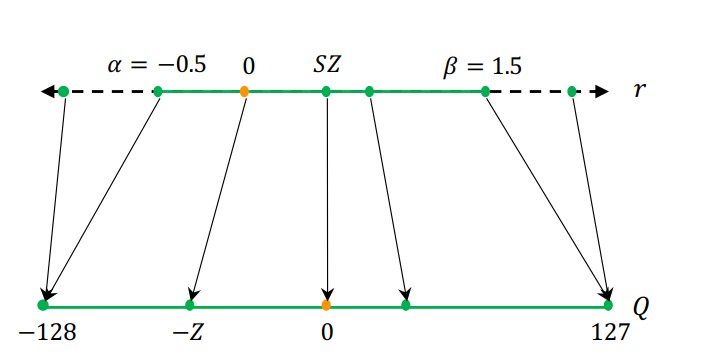
\includegraphics[width=5in,height=2.46875in]{img/3/quant.png}
    \caption{Cuantización INT8 en el intervalo $[-0.5,1.5$]. Extraído de \cite{quant_survey}}
    \label{fig:quant}
\end{figure}

En el proceso de cuantización tenemos presente dos parámetros para cada
uno de los tensores:

\textbf{Escala ($S$)}: Es un número decimal que nos permite escalar los
valores entre un número real y uno cuantizado.

\textbf{Zero Point ($Z$):} Es un número dentro del intervalo de cuantización.
Nos indica el valor del 0 real en valores cuantizados.

Estos valores son calculados a partir de analizar las distribución de los distintos tensores y activaciones.

\begin{equation}
    S = \frac{\beta - \alpha}{\beta_q - \alpha_q}    
\end{equation}

\begin{equation}
    Z = \left\lceil\frac{\beta\alpha_q - \alpha\beta_q}{\beta-\alpha}\right\rfloor
\end{equation}



En el caso de la distribución de valores reales, debemos conocer el valor mínimo
($\alpha$) y el máximo ($\beta$) del tensor/distribución a cuantizar.\footnote{Existen otras técnicas más avanzadas que tienen en cuenta la existencia de outliers en la distribución, lo que puede aumentar el ruido de cuantización.} 

Para los tensores cuantizados, $\alpha_q$ y $\beta_q$ se corresponden con el mínimo y el máximo de
los tipos de datos, para INT8,  $\alpha_q = -128$ y $\beta_q = 127$.

Una vez obtenidos $S$, $Z$, $\alpha_q$ y $\beta_q$, ya podemos cuantizar o decuantizar los distintos tensores con la siguiente ecuación.\footnote{La operación de decuantización debe tener en cuenta los errores de redondeo y clip si se quiere recuperar $x$. Nosotros no tenemos en cuenta los errores ya que no afectan al rendimiento de la red.}
\begin{equation}
    x_q = clip(round(\frac{1}{s}x + z), \alpha_q, \beta_q)
\end{equation}


Siendo clip una operación de saturación que impide que resultado de la cuantización sea un valor sea menor que $\alpha_q$ o mayor que $\beta_q$.
En la figura \ref{fig:quant} esta operación se ve reflejada en los valores que están fuera del intervalo $[\alpha,\beta]$


\hypertarget{tecnicas-de-cuantizacion}{%
\subsection{\texorpdfstring{Técnicas de Cuantización
}{Técnicas de Cuantización }}\label{tecnicas-de-cuantizacion}}
Existen dos técnicas de cuantización post entrenamiento:
\subsubsection{Fake Quantization o Cuantización Dinámica:}
Los pesos se almacenan en un tipo de datos inferior, pero los parámetros
de cuantización $S$ y $Z$ se calculan en tiempo de inferencia.
\subsubsection{Fixed Quantization:}
En este caso los parámetros de la cuantización se calculan durante el
proceso de cuantización. Este tipo de cuantización requiere utilizar un
\textbf{conjunto de datos representativo} \textbf{de entrada} durante el
proceso de cuantizado, con el que se calcularán los parámetros de
cuantización de cada tensor.

\hypertarget{resultados-de-la-cuantizaciuxf3n}{%
\subsection{Resultados de la
cuantización}\label{resultados-de-la-cuantizaciuxf3n}}
\begin{figure}
    \centering
    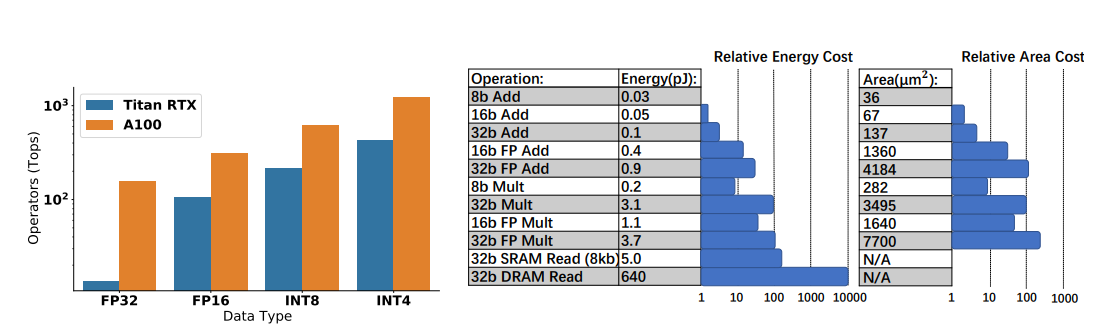
\includegraphics[width=5in,height=1.45833in]{img/3/quant_res.png}
    \caption{Resultados del coste de la operaciones dependiendo del tipo de dato de una red neuronal. Extraído de \cite{quant_survey}}
    \label{fig:quant-res}
\end{figure}

Si bien este proceso es muy eficiente como se puede observar en la figura \ref{fig:quant-res}, tiene un inconveniente muy
importante, y es que la salida de una neurona está limitada a tantos
valores como como el tipo de dato que utilicemos. En el caso de INT8 o UINT8, una neurona solo puede tener 256 valores distintos en su salida.

Por otro lado, esto no debería ser ningún problema si trabajamos con
tareas de clasificación con pocas etiquetas, pero es importante comprobar con un conjunto de
prueba que la precisión de la red no se ha visto afectada por la
cuantización.


\hypertarget{ensembles-ova-y-ovo}{%
\section{Ensembles, OVA y OVO}\label{ensembles-ova-y-ovo}}

Existen múltiples técnicas para clasificar conjuntos de datos con múltiples
clases. En este aparatado vamos a comentar dos tipos de ensembles que
unen varios clasificadores binarios para obtener un único clasificador
multiclase.
En algunas situaciones, los ensembles binarios pueden ser mucho más robustos que un único clasificador multietiqueta. 
Hemos planteado el uso de ensembles para mejorar el rendimiento de los distintos clasificadores de clasificación de géneros y estados de ánimo.

\begin{figure}[h]
    \centering
    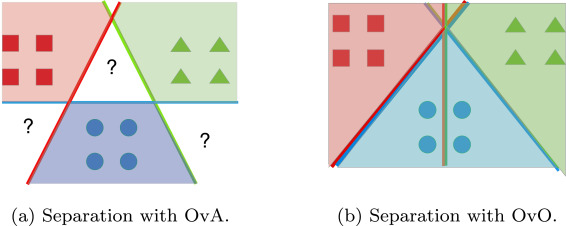
\includegraphics[]{img/3/ova-ovo.jpg}
    \caption{Comparación entre OVA y OVO. Extraído de \cite{OVA_vs_OVO}}
    \label{fig:ova-ovo}
\end{figure}


\hypertarget{one-vs-all}{%
\subsection{One vs All}\label{one-vs-all}}

El ensemble One vs All (OVA) divide un problema con $N$ clases en $N$
clasificadores binarios. Cada uno de estos clasificadores se encarga de
identificar si una entrada se corresponde con una clase (1) o no (0). En
este caso, es importante que el clasificador no esté calibrado, es decir,
su salida debe asemejarse con la confianza del resultado, ya que, si nos
encontramos con un conflicto entre varios clasificadores base por tener
la misma salida, no vamos a poder predecir la clase correctamente.

\textbf{Ejemplo Red Neuronal Binaria}

Si utilizamos la \textbf{función de activación escalón} en la neurona de
salida de nuestra red neuronal, nos encontramos con que la salida
únicamente tiene dos valores, 0 y 1, por lo que no conocemos la
confianza de la predicción.

Por otro lado, si utilizamos la \textbf{función sigmoide} \eqref{eq:sigmoid} como función
de activación, nos encontramos con una función cuyo recurrido son
valores reales en el intervalo {[}0, 1{]}, por lo que podríamos
considerar que la salida es la confianza que tiene la red ante una
predicción.

\hypertarget{one-vs-one}{%
\subsection{One vs One}\label{one-vs-one}}

El ensemble One vs One (OVO), a diferencia del ensemble OVA, busca una
clasificación más robusta entrenando un mayor número de clasificadores\\
Si en el ensemble OVA únicamente lidiábamos con las colisiones teniendo en cuenta
la confianza, el ensemble OVO es capaz de conocer si un dato pertenece a
una clase o a otra, ya que cada uno de los clasificadores se entrena con
un subconjunto de datos formado solo por dos clases\footnote{Clasificación Binaria}.

En este caso, tenemos que entrenar $L = K(K-1)/2$ clasificadores binarios,
un número mucho más grande que en el ensemble OVA, por lo que el coste
en memoria y tiempo de entrenamiento es mucho mayor.

En el caso del ensemble OVO, el clasificador base no solo no tiene que
estar correctamente calibrado, sino que además las salidas deben estar
comprendidas en el intervalo {[}-1, 1{]}, siendo -1 la clase A, 1 la
clase B, y 0 el valor correspondiente la clase desconocida.

Para evaluar la salida de todos los clasificadores, debemos construir
una matriz $N \times L$ (\ref{fig:matrix-ovo}), que permita convertir el vector $L$ a un vector con $N$
elementos con la confianza de cada clase. Cada fila de la matriz se
corresponde con cada clase, y debemos asignar el mismo valor (1 o -1)
que hemos utilizado como etiqueta durante el entrenamiento
\begin{figure}[h]
    \centering
    $$
    M = 
    \begin{bmatrix}
    1 & 1 & 1 & 0 & 0 & 0 \\
    -1 & 0 & 0 &  1 & 1 & 0 \\
    0 & -1 & 0 & -1 & 0 & 1 \\
    0 & 0 & -1 & 0 & -1 & -1 
    
    \end{bmatrix}
    $$
    \label{fig:matrix-ovo}
    \caption{Matriz para N=4}
\end{figure}


Haremos una multiplicación de matrices entre la matriz y la salida de
los clasificadores, obteniendo una matriz N x L con la probabilidad de
cada clase. Como hemos utilizado valores en el intervalo {[}-1, 1{]}
como salida de cada clasificador, al realizar la multiplicación de
matrices nos encontraremos con que únicamente tenemos valores positivos.\\
Si sumamos todas las columnas, de la matriz anterior obtendremos la
confianza del ensemble para cada uno de los datos.


\section{Ball Tree}\label{ball_tree}
Un ball tree o árbol de bolas es una estructura de datos jerárquica utilizada para la gestión de vecindarios de instancias. Esta estructura de datos permite conocer de una manera eficiente el vecindario de una instancia.

Se ha utilizado esta estructura de datos para buscar los vecinos más cercanos a una canción, como una posible técnica para identificar canciones similares.

Para construir un árbol de bolas, las instancias se dividen en dos clusters o bolas\footnote{También conocido como esferas o hiperesferas}, siendo cada cluster una rama del árbol. Los cluseters son calculados de la siguiente manera:
\begin{enumerate}
    \item Se selecciona una instancia aleatoria
    \item Se busca la instancia más alejada a la instancia seleccionada
    \item Se calcula el punto intermedio que hay entre las dos instancias
    \item Se divide el espacio en dos mediante un hiperplano
    \item Se calculan los centroides de los clusters que hay en cada división.
    \item Se crea una esfera que cubra todos las instancias de cada clúster
\end{enumerate}\\
Repetimos el proceso para cada una de las esferas hasta alcanzar el número de instancias por hoja buscado (Por defecto son 40 instancias por hoja en SKLearn).

Hecho esto, podemos consultar rápidamente el vecindario correspondiente a una nueva instancia a partir de los centroides más cercanos a nuestra instancia, sin necesidad de explorar todos los vecinos posibles. 

\section{Sistemas de Recomendación}
Un sistema de recomendación es un algoritmo que intenta predecir la valoración o interés que puede tener un usuario ante un nuevo elemento. Existen dos tipos principales de sistemas de recomendación, los sistemas basados en contenido y los filtrados colaborativos. 

Los sistemas basados en contenido realizan recomendaciones a partir de las etiquetas o metadatos del elemento. Se ha usado este tipo de sistema de recomendación para recomendar canciones similares basados en características extraídas del audio de las canciones. Se ha explorado el uso de estos sistemas en el apartado \ref{recomend_contenido}.

Los sistemas colaborativos tienen en cuenta las valoraciones o gustos de otros usuarios para realizar las recomendaciones.
Estos sistemas funciona a partir de la creación de una matriz usuario/elemento, en la que se almacena las valoraciones de los usuarios. De esta matriz se puede extraer una matriz usuario/usuario con la similitud que hay entre los gustos de los distintos usuarios. Para estos sistemas de filtrado se recomienda usar Suprise \ref{scikit-surprise}, una biblioteca que implementa una gran variedad de algoritmos para trabajar con sistemas colaborativos. Se ha usado este sistema de recomendación para rellenar playlists de usuario, como explora el apartado \ref{recomend_colab}.
\capitulo{4}{Técnicas y Herramientas}

%Este capítulo tiene la finalidad de resaltar las distintas tecnologías, técnicas y herramientas que han sido utilizadas a lo largo del desarrollo del proyecto. 
\vspace{-0.35cm}



\hypertarget{tecnologuxedas-y-dependencias}{%
\section{Tecnologías y
Dependencias}\label{tecnologuxedas-y-dependencias}}

En este apartado se van a mencionar las diferentes tecnologías, bibliotecas y frameworks que han sido utilizados para construir el frontend y los dos servidores web de SpotMyFM.

\hypertarget{frontend}{%
\subsection{Frontend}\label{frontend}}
El frontend es un cliente web ajeno a Spotify dedicado a expandir la funcionalidad de la plataforma mediante su API pública.

\hypertarget{typescript}{%
\subsubsection{\texorpdfstring{Typescript
}{Typescript }}\label{typescript}}

Typescript es un superset del lenguaje de programación Javascript, por
lo que cualquier código escrito en Javascript puede ser utilizado como
código Typescript. La principal característica de este superset es la
inclusión de un sistema de tipado estático fuerte.

Para el desarrollo de los componentes se ha utilizado TSX (Typescript
Syntax Extensions), esta extensión de Typescript permite generar HTML
junto con Typescript, facilitando la generación de HTML dinámico.\\
Estas extensiones de lenguaje no están reflejadas en el estándar de
ECMAscript, por lo que es necesario utilizar un transpilador que
convierta estas extensiones en código Javascript.

Se ha tenido en cuenta utilizar JavaScript y JSX como alternativa.

Página oficial: \href{https://www.typescriptlang.org/}{https://www.typescriptlang.org/}

\hypertarget{nextjs}{%
\subsubsection{NextJS}\label{nextjs-front}}

NextJS es un framework de Javascript compatible con Typescript que
permite construir interfaces. NextJS está construido sobre la biblioteca
ReactJS, y añade una gran variedad de características como:

\begin{itemize}
\itemsep0em 
\item
  Rutas o Páginas (/home, /about, etc)
\item
  Server Side Rendering
\item
  Rutas de API basadas en NodeJS
\item
  Empaquetamiento sin configuración
\item
  Api de internacionalización
\end{itemize}

ReactJS es una biblioteca de desarrollo de interfaces web que incluye un
Virtual DOM que permite montar y desmontar componentes JSX en el DOM de
manera transparente.

Se ha tenido en cuenta utilizar ReactJS como una alternativa.

Página oficial: \href{https://nextjs.org/}{https://nextjs.org/}

\subsection{i18next y Next Translate}\label{i18n}
Se ha utilizado la biblioteca i18next junto con el adaptador Next Translate para la internacionalización del frontend. 

i18next es una mejora sobre i18, una de las biblioteca de internacionalización más utilizadas del mundo. Next Translate incluye un Hook \begin{verbatim}
    useTranslation()
\end{verbatim} que permite obtener el código del idioma actual ("es", "en"), y un objeto que obtiene las traducciones a partir de su identificador. 

Las traducciones se almacenan en ficheros .json, en el que la clave es el identificador de la traducción y el valor es el string traducido. 



\hypertarget{tailwind-css}{%
\subsubsection{\texorpdfstring{Tailwind CSS
}{Tailwind CSS }}\label{tailwind-css}}

Tailwind CSS es una biblioteca de generación de hojas de estilo CSS de
código abierto muy interesante. Su principal filosofía es la de la
creación de clases de utilidad dinámicas con las que podemos seguir
buenas prácticas de CSS. Esta biblioteca está acompañada con un
preprocesador que se encarga de generar y optimizar las stylesheets a
partir de las clases que hemos utilizado.

Una de sus características más interesantes es la generación de clases
de utilidad con variantes que permiten cambiar el estilo dependiendo de
algunos condicionales.\\
Algunas de estas variantes de estado pueden ser:

\begin{itemize}
\itemsep0em 
\item
  hover:\textless clases de utilidad\textgreater{} estilo cuando el
  ratón está encima de un elemento
\item
  sm:\textless clases de utilidad\textgreater{} estilo cuando el ancho
  del viewport es mayor a 640px
\item
  dark:\textless clases de utilidad\textgreater{} estilo a aplicar
  cuando estamos utilizando el modo oscuro
\item
  \ldots{}
\end{itemize}

Por último, esta biblioteca permite declarar nuestras propias paletas de
colores, variantes de estado, clases de utilidad, etc, por lo que
podemos expandirla manualmente.

Página oficial: \href{https://tailwindcss.com/}{https://tailwindcss.com/}


\hypertarget{twin-macro-y-styled-components}{%
\subsubsection{Twin Macro y Styled
Components}\label{twin-macro-y-styled-components}}

En la actualidad, debido a las limitaciones de las hojas de estilo en
cascada, existen múltiples métodos de escribir estilos CSS, como los ficheros .css, estilos en línea, estilos como componentes o CSS in JS.


Para esta aplicación hemos utilizado el paradigma CSS in JS, que nos
permite declarar los estilos CSS en el propio código de la aplicación.
La principal ventaja de este paradigma es que podemos modificar los
atributos CSS directamente desde nuestro código.

Twin macro es un adaptador de distintas bibliotecas \textbf{CSS in JS},
que permite estilar mediante TailwindCSS con bibliotecas CSS in JS como
PostCSS, Emotion o Styled Componets.

En este caso hemos escogido la biblioteca \textbf{Styled Coponentes},
que nos permite declarar o estilar componentes de ReactJS.

Repositorio oficial: \href{https://github.com/ben-rogerson/twin.macro}{Twin Macro}\\
Página oficial: \href{https://styled-components.com/}{https://styled-components.com/}

\hypertarget{zustand}{%
\subsubsection{Zustand}\label{zustand}}

Zustand es una biblioteca de código abierto para la gestión de estado de
React basada en hooks. Esta biblioteca permite declarar stores (espacios
de almacenaje de estados) en los que podemos almacenar datos y sus
operaciones que deseamos compartir entre varios componentes.

En el caso de la aplicación, hemos utilizado esta biblioteca para
almacenar estados globales, como el estilo de la web, la pestaña que
tenemos activa o instancias únicas de los distintos clientes REST de la
aplicación.

Página oficial: \href{https://zustand.surge.sh/}{https://zustand.surge.sh/}

\hypertarget{dexiedb}{%
\subsubsection{DexieDB}\label{dexiedb}}

DexieDB o DexieJS es un wrapper de IndexedDB, una \textbf{base de datos} NO-SQL
que se encuentra en todos los navegadores modernos.

Este wrapper, a parte de contener toda la funcionalidad de DexieDB, nos
permite declarar los esquemas de la base de datos junto sus distintas
operaciones y comprobaciones.\\
DexieDB es compatible con Typescript, por lo que permite operar las
tablas con supervisión de tipos.

Página oficial: \href{https://dexie.org/}{https://dexie.org/}

\hypertarget{jest}{%
\subsubsection{Jest}\label{jest}}

Jest es una biblioteca de código abierto de pruebas unitarias
desarrollada por Facebook. Esta biblioteca tiene una gran variedad de
características, como Mocking, compatibilidad con código asíncrono,
compatibilidad con React, Typescript, Node, etc.

Una de las principales ventajas de Jest son las extensiones de su
comunidad. En este caso se ha utilizado la extensión \textbf{React
Testing Library}, una extensión que permite renderizar internamente
componentes de React y hacer comprobaciones sobre el DOM Virtual.

Página oficial: \href{https://jestjs.io/}{https://jestjs.io/}

\hypertarget{cypress}{%
\subsubsection{Cypress}\label{cypress}}

Cypress es un framework de pruebas punto a punto de código abierto.
Cypress es muy similar a Selenium, ambas realizan pruebas automatizadas
sobre un navegador físico, pero Cypress es mucho más sencillo de
configurar.

Algunas de las características más relevantes de Cypress son: velocidad de ejecución, grabación de los tests fallidos, tamaño de viewport variable, ejecución headless y compatibilidad con Github Actions \ref{github-actions}

Página oficial: \href{https://www.cypress.io/}{https://www.cypress.io/}

\hypertarget{otras}{%
\subsubsection{Otras:}\label{otras}}

\begin{itemize}
\item
  \textbf{Recharts}: Es una biblioteca de código abierto para React que
  permite generar gráficas interactivas.
  Página oficial: \href{https://recharts.org/}{https://recharts.org/}
\item
  \textbf{React Icons}: Una colección de iconos vectoriales que junta
  múltiples bibliotecas de iconos.
  Página oficial: \href{https://react-icons.github.io/react-icons}{https://react-icons.github.io/react-icons}
\item
  \textbf{Framer Motion}: Biblioteca de código abierto que permite
  añadir animaciones que dependen de los estados internos de un
  componente.
  Página oficial: \href{https://www.framer.com/motion/}{https://www.framer.com/motion/}
\end{itemize}

\hypertarget{backend-nextjs}{%
\subsection{Servidor NextJS}\label{backend-nextjs}}
El servidor de NextJS se encarga de la gestión de la base de datos, inicio de sesión, generación de tokenes de identificación JWT y de la comunicación con el servidor de recuperación de información musical. 

\hypertarget{nextjs-api-rest}{%
\subsubsection{NextJS API REST}\label{nextjs-api-rest}}

NextJS incluye una API REST funcional basada muy simple basada en
Node/Express. Esta API tiene como principal objetivo apoyar al
funcionamiento del cliente en dos situaciones.

\begin{itemize}
\item
  Renderizar en el servidor (SSR)\footnote{Server Side Rendering} elementos dinámicos de la web. Como
  por el ejemplo vistas individuales para usuarios registrados.
\item
  Trabajar con peticiones que requieran autenticación.
\end{itemize}

En este api, un endpoint se define como un fichero .ts/.js que recibe
dos objetos, la petición HTTP y la respuesta HTTP. Como cada endpoint se
corresponde con un fichero único, la API permite el paradigma de cloud
computing FaaS (Functions as a Service), en el que cada función puede
actuar como un pequeño microservicio.

Cada endpoint puede alojarse de manera independiente en plataformas
como Cloudflare Workers o AWS Lambda.

\hypertarget{jwt}{%
\subsubsection{JWT}\label{jwt}}

JWT (Json Web Tokens) es un método de representación de tokens en
formato json basado en el estándar RFC 7519. Los tokens están formados
por tres segmentos:

\begin{itemize}
\item
  Cabecera: Es un json serializado en base64 que incluye el tipo del
  token y el algoritmode firma utilizado (RSA, SHA256, etc)
\item
  Payload: Es otro json serializado en base 64 que incluye los
  contenidos del token.
\item
  Firma de verificación: Firma hash generada a partir de una clave
  privada y los campos anteriores. Permite comprobar que el payload no
  ha sido modificado.
\end{itemize}

Una vez construidos y serializados los 3 segmentos, estos son
concatenados mediante un punto (``.'') y pueden ser deserializados por
cualquier receptor.

Se han utilizado estos tokenes para poder identificar al usuario y sus operaciones permitidas. Este token se envía a la API para todas las peticiones, y a diferencia de identificar al usuario con su token de usuario de Spotify, al solo comprobar la validez de la firma no se tienen que enviar más peticiones a Spotify, mejorando la latencia de cada endpoint. 

Biblioteca específica utilizada: \href{https://www.npmjs.com/package/jsonwebtoken}{https://www.npmjs.com/package/jsonwebtoken}

\hypertarget{dynamodb-y-dynamoose}{%
\subsubsection{DynamoDB y Dynamoose}\label{dynamodb-y-dynamoose}}

\textbf{DynamoDB} es una base de datos NO-SQL basada en documentos clave
valor desarrollada por Amazon para AWS, su plataforma de Cloud
Computing.\\
Algunas características de esta base de datos son:

\begin{itemize}
\item
  Capacidad bajo demanda
\item
  Base de datos sin servidor (No utiliza sockets / conexiones físicas,
  por lo que es apta para ser accedida por la arquitectura sin servidor,
  como CaaS o FaaS.
\item
  Compatibilidad con AWS OpenSearch (E lasticSearch)
\item
  Copias de seguridad
\item
  Replicas
\item
  Transacciones ACID
\end{itemize}

Además, DynamoDB está incluida en el plan gratuito de AWS, y ofrece 25GB
de por vida.

\textbf{Dynamoose} es una herramienta de modelado de DynamoDB que permite utilizar las distintas características de AWS
desde un api de alto nivel.

La principal ventaja de Dynamoose es que permite modelar los esquemas de
la base de datos en Typescript/Javascript. Estos esquemas serán
validados por Dynamoose antes de crear, modificar o leer documentos.

\textbf{Otras Bases de datos planteadas}

    \begin{table}[h]
    \resizebox{\textwidth}{!}{%
    \begin{tabular}{@{}llllll@{}}
    \toprule
                                                                                                    & Firestore                                                                & MongoDB       & Supabase    & DynamoDB         & Heroku        \\ \midrule
    \textbf{Tipo}                                                                                   & Documentos                                                               & Documentos    & Relacional  & Documentos       & Relacional    \\
    \textbf{Capacidad}                                                                              & 1GB                                                                      & 0.5GB         & 0.5GB       & 25GB             & 1000 filas    \\
    \textbf{Lim.   Peticiones}                                                                      & \begin{tabular}[c]{@{}l@{}}50k R/doc/day  \\ 20k W/ doc/day\end{tabular} & No hay        & No Hay      & 200M R+W /mes    & No            \\
    \textbf{Self-hosted}                                                                            & No                                                                       & Si            & Si          & NO               & Si            \\
    \textbf{SSL}                                                                                    & Si                                                                       & Si            & Si          & Si               & Si            \\
    \textbf{Escalable}                                                                              & Si                                                                       & Si            & Si          & Si               & Si              \\
    \textbf{Pausa}                                                                                  & No                                                                       & No            & Si (7 días) & No               & Si (7 días)   \\
    \textbf{\begin{tabular}[c]{@{}l@{}}ORM/   Bussiness Logic / \\ Model / Validation\end{tabular}} & No                                                                       & Si (Mongoose) & No          & Si   (Dynamoose) & Si (Postgres) \\
    \textbf{Editor}                                                                                 & Si                                                                       & Si            & Si          & Si (De pago)     & Si            \\ \bottomrule
    \end{tabular}%
    }
    \end{table}

Página oficial de DynamoDB: \href{https://aws.amazon.com/es/dynamodb/}{https://aws.amazon.com/es/dynamodb/}

Página oficial de Dynamoose: \href{https://dynamoosejs.com/}{https://dynamoosejs.com/}

\hypertarget{backend-mir}{%
\subsection{Backend MIR}\label{backend-mir}}

El backend de \textbf{recuperación de la información musical} está basando en
Python 3.8 y permite obtener las etiquetas y canciones similares a partir de un fichero de audio.

\hypertarget{fastapi}{%
\subsubsection{FASTAPI}\label{fastapi}}

FastAPI es un framework web diseñado para construir APIs con Python
3.6+.

La principal característica de FastAPI es que utiliza el sistema de
sugerencia de tipos de Python para validar las distintas peticiones
HTTP.

Este sistema permite asignar un tipo de forma estática a una variable,
estos tipos son ignorados en tiempo de ejecución, pero pueden se
utilizados para documentar o como comprobación en tiempo de desarrollo
mediante un linter.
\begin{verbatim}
foo: int = 1 # No error
foo: int = "bar" # typechcking error  
\end{verbatim}


Además de validar las peticiones de nuestra aplicación, FastAPI genera
automáticamente \textbf{documentación interactiva} para cada endpoint
con \textbf{OpenAPI y Redocs}.

Por último, FastAPI utiliza el api de \textbf{corrutinas} de Python
basada en la sintaxis Async/Await. Cada uno de los endpoints puede ser
definido como una corrutina asíncrona con la que podemos esperar a
ejecución de otras corrutinas utilizando la palabra clave await,
facilitando el uso de bibliotecas concurrentes.

Página oficial: \href{https://fastapi.tiangolo.com/}{https://fastapi.tiangolo.com/}

\hypertarget{aiohttp}{%
\subsubsection{AIOHTTP}\label{aiohttp}}

\textbf{aiohttp} es una biblioteca de Python basada en \textbf{requests}
que permite realizar \textbf{peticiones http concurrentes}. aiohttp
utiliza el api de corrutinas, por lo que puede sen consumida
directamente desde un endpoint de FastAPI.

Página oficial: \href{https://docs.aiohttp.org/en/stable/}{https://docs.aiohttp.org/en/stable/}


\hypertarget{onnx-runtime-python}{%
\subsubsection{ONNX Runtime Python}\label{onnx-runtime-python}}

\textbf{ONNX Runtime} \cite{onnxruntime} es una biblioteca de código abierto mantenida por
Facebook y Microsoft. Esta biblioteca implementa múltiples motores de
inferencias compatibles con el estándar \textbf{Open Neural Network
eXchange (ONNX)}, un estándar que busca la interoperabilidad de modelos
neuronales a partir de una \textbf{representación intermedia (IR).}

La filosofía de ONNX es que un modelo neuronal pueda ser utilizado en
cualquier hardware independientemente de su representación interna, para
ello existen una serie herramientas para convertir y optimizar modelos
basados en Pytorch, Keras, Caffé, etc en representación intermedia.

Un modelo IR puede ser utilizado en múltiples \textbf{plataformas}, como Windows, Linux, Android, Ios, navegadores web, \ldots, e independientemente de la arquitectura del procesador (X86, X64, ARM, \ldots).

La principal ventaja de ONNX es su compatibilidad con diferentes lenguajes de programación, ya que permite inferir modelos desde C++, Python, Java, C\# o incluye NodeJS/JS/TS.
Por último, ONNX incluye aceleración por hardware con una gran cantidad de APIs, como Nvidia CUDA, Nvidia TensorRT, Intel OpenVINO, Windows DirectML, \ldots.

Página oficial: \href{https://onnx.ai/}{https://onnx.ai/}

\hypertarget{librosa}{%
\subsubsection{Librosa}\label{librosa}}

Librosa es una biblioteca de Python enfocada al análisis de audio y
música. Esta biblioteca está basada en Scipy y es muy utilizada a la
hora de trabajar con sonido en Python.

Esta biblioteca incluye todos los componentes necesarios para poder
trabajar con audio, desde la lectura / creación de ficheros de audio,
conversión entre formatos, muestreo, visualización y extracción de
características.

En este apartado del proyecto utilizamos librosa para leer ficheros wav
y extraer algunos datos como los MFCCs \ref{coeficientes-cepstrales-en-las-frecuencias-de-mel}, Tempo o el Beat:

Se ha tenido en cuenta el uso de Torch Audio para las tareas de
preprocesamiento.

Página oficial: \href{https://librosa.org/}{https://librosa.org/}

\hypertarget{ffmpeg}{%
\subsubsection{FFMPEG}\label{ffmpeg}}

FFMPEG es conjunto de bibliotecas de \textbf{alto rendimiento} que
permiten trabajar con datos multimedia (ficheros y streams de vídeo,
audio, imágenes, etc). FFMPEG permite grabar, editar, convertir,
transcodificar o escalar datos multimedia.

El servidor de recuperación de información musical utiliza FFMPEG para convertir y muestrear ficheros .mp3 a
.wav en 22050HZ, ya que es la representación de onda en formato .wav es la misma con la que trabaja Librosa. 
Librosa es compatible con formatos .mp3, pero su implementación no es tan eficiente como la de FFMPEG.

Página oficial: \href{https://ffmpeg.org/}{https://ffmpeg.org/}

\hypertarget{sklearn}{%
\subsubsection{Sklearn}\label{sklearn}}

Sklearn \cite{scikit-learn} es una biblioteca basada en SciPy \cite{2020SciPy-NMeth} diseñada para tareas de
aprendizaje automático.

Incluye una gran variedad de algoritmos para tareas de clasificación,
regresión, clustering, reducción de dimensionalidad, selección de modelo
o preprocesado.

Este backend utiliza dos componentes de Sklearn:

\begin{itemize}
\itemsep0em 
\item
  \textbf{BallTree}: Utilizado para encontrar los vecinos más cercanos a
  un dato.
\item
  \textbf{MinMaxScaler}: Utilizado para normalizar la entrada al
  BallTree
\end{itemize}

Página oficial: \href{https://scikit-learn.org/}{https://scikit-learn.org/}

\subssubection{Knime}\label{knime}
Knime o Konstanz Information Miner es una herramienta de código abierto usada en minería de datos y aprendizaje automático. Esta herramienta permite construir de manera visual mediante nodos interconectados flujos de trabajo para visualizar, modificar y analizar datos.
Se ha utilizado KNime para el análisis de los distintos conjuntos de datos. 

Página oficial: \href{https://www.knime.com/}{https://www.knime.com/}

\hypertarget{scikit-surprise}{%
\subsubsection{Scikit Surprise}\label{scikit-surprise}}

Surprise \cite{supriselib} es una biblioteca de código abierto especializada en sistemas
de recomendación colaborativos.

El funcionamiento de esta biblioteca es muy simple, ya que permite
generar la matriz de recomendación a partir de una tabla con tres columnas, el ID del usuario, el ID del Elemento y un escalar con la votación del usuario. 

Surprise implementa una gran variedad de algoritmos, como SVD o NMF
utilizados en descomposición de matrices, y otros más tradicionales como
KNN, Co Clustering o Slope One.

Por otro lado, Surprise además implementa un sistema de evaluación de
recomendaciones, que valora la precisión del modelo a partir de intentar
completar recomendaciones para usuarios incompletos.

Página oficial: \href{http://surpriselib.com/}{http://surpriselib.com/}

\hypertarget{herramientas-y-servicios}{%
\section{Herramientas y Servicios}\label{herramientas-y-servicios}}

\hypertarget{kaggle}{%
\subsection{Kaggle}\label{kaggle}}

Kaggle es una comunidad de ciencia de datos en la que se publican
conjuntos de datos y competiciones.

Uno de los servicios que incluye Kaggle es \textbf{Code}, un servicio
para publicar y ejecutar notebooks que utilicen el Dataset con aceleración por hardware. \\
En este caso se ha utilizado Kaggle para publicar los datasets y
entrenar los modelos de forma remota. Se ha planteado el uso de Google Cloud Notebooks y Google Colab para el
entrenamiento de los modelos.

Página oficial: \href{https://www.kaggle.com/}{https://www.kaggle.com/}

\hypertarget{tensorflow-keras}{%
\subsection{Tensorflow Keras}\label{tensorflow-keras}}

Tensorflow \cite{tensorflow2015-whitepaper} es una biblioteca de código abierto destinada a el
entrenamiento e inferencia de modelos neuronales. Tensorflow está
pensada para ser usada con Python, pero es compatible con otros
lenguajes como C++ o incluso JavaScript.

Keras es una API de Tensorflow para Python que simplifica la
implementación y entrenamiento de redes neuronales mediante Tensorflow.

Se ha planteado el uso de Pytorch como alternativa a Tensorflow Keras.

Página oficial: \href{https://www.tensorflow.org/}{https://www.tensorflow.org/}



\hypertarget{onnx-tensorflow-converter-y-onnx-quantizer}{%
\subsection{ONNX Tensorflow Converter y ONNX
Quantizer}\label{onnx-tensorflow-converter-y-onnx-quantizer}}

ONNX Tensorflow Converter \cite{onnxruntime} es una herramienta de línea de comandos que
permite convertir un modelo de Tensorflow en un modelo del estándar
ONNX.

ONNX Quantizer es una biblioteca de Python que permite cuantizar modelos
de ONNX. Esta herramienta es compatible tanto con la cuantización
dinámica como con la estática.

Ambas herramientas forman parte del proyecto de código abierto ONNX,
mantenido por Microsoft y Facebook.

Se ha tenido en cuenta el uso de TFLITE para cuantizar e inferir los modelos,
pero este motor únicamente está optimizado para dispositivos móviles
(ARM).

Página oficial: \href{https://onnxruntime.ai/}{https://onnxruntime.ai/}

\hypertarget{github}{%
\subsection{Github}\label{github}}

Github es una plataforma para alojar repositorios git. Esta plataforma
permite crear y compartir repositorios públicos y privados, utilizar
ramas, crear y gestionar pull requests, y muchas otras características
como la creación de flujos de trabajo con Github Actions o el control de
dependencias con Dependabot.

Se ha utilizado Github y su sistema de Issues para el control de
versiones del proyecto y la planificación temporal del proyecto.

Repositorio del proyecto \href{https://github.com/JorgeRuizDev/SpotMyFM}{https://github.com/JorgeRuizDev/SpotMyFM}

\hypertarget{zenhub}{%
\subsection{Zenhub}\label{zenhub}}

Zenhub es una herramienta de gestión de proyectos que intenta integrarse
con Github. Esta biblioteca presenta un tablero Kanban en el que podemos
encontrarnos cada una de las tareas del propio repositorio.

Zenhub, además tiene un sistema de sprints, épicas y puntos de historia
con el que podemos gestionar proyectos utilizando la metodología Scrum.

Página oficial: \href{https://www.zenhub.com/}{https://www.zenhub.com/}

\hypertarget{dependabot}{%
\subsection{\texorpdfstring{Dependabot
}{Dependabot }}\label{dependabot}}

Dependabot es un servicio integrado en Github que permite analizar un
respositorio en busca de brechas de seguridad.\\
Este servicio analiza el código en busca de \textbf{filtraciones de
claves o tokens secretos}, y como su propio nombre indica, analiza las
\textbf{dependencias del proyecto} en busca de dependencias vulnerables.\\
Si Dependabot detecta una vulnerabilidad en el proyecto, este intentará
corregirla y publicará una \textbf{Pull Request} con la vulnerabilidad
solucionada.

\hypertarget{docker}{%
\subsection{Docker}\label{docker}}

Docker es una plataforma que permite crear y desplegar contenedores. Un
contenedor es un ``paquete'' que contiene todos los requisitos para que
una aplicación se pueda ejecutar en un entorno aislado, como el binario
de la aplicación, dependencias, configuraciones de red, etc.

Estos contenedores pueden ser considerados una pequeña máquina virtual,
ya que cada contenedor tiene su propio sistema de ficheros, unidades, o
LAN, pero a diferencia de una máquina virtual, el contenedor se ejecuta
sobre el \textbf{Docker Engine} y no sobre un \textbf{hipervisor.}

En este caso se ha utilizado Docker para crear los contenedores con los
que poder desplegar las aplicaciones de NextJS y FastAPI.

Página oficial: \href{https://docs.docker.com/}{https://docs.docker.com/}

\hypertarget{github-copilot}{%
\subsection{Github Copilot}\label{github-copilot}}

Github Copilot es un servicio online que permite sugerir cambios o
implementaciones de código basado en el contexto actual del fichero que
estamos editando. Copilot se integra con el editor (VSCODE) o IDE
(Webstorm) y necesita conexión a internet para procesar las sugerencias.

La principal ventaja de Copilot frente a otros servicios de
autocompletado como Intellisense es que Copilot utiliza los tipos de
datos, comentarios, estilo del código, nombres de variables y nombres de
funciones para sugerir cambios o implementaciones.

Página oficial: \href{https://github.com/features/copilot}{https://github.com/features/copilot}

\hypertarget{github-actions}{%
\subsection{Github Actions}\label{github-actions}}

Github Actions es un servicio integrado en Github que permite ejecutar
flujos de trabajo sobre un repositorio a partir de distintos estados.

En este caso, se han programado las siguientes acciones para cada push
al repositorio:

\begin{itemize}
\itemsep0em 
\item
  \textbf{Prettier}: Aplica el formateador de código Prettier a todos
  los ficheros compatibles (Typescript, Javascript, JSON, CSS, etc)
\item
  \textbf{Integración Continúa}: Asegura que el proyecto se compila
  correctamente y ejecuta las pruebas unitarias sobre las distintas
  clases del proyecto.
\item
  \textbf{Cypress:} Ejecuta las pruebas punto a punto sobre el
  despliegue de la aplicación.
\end{itemize}\\
Se ha considerado el uso de los servicios TravisCI y CircleCI.\\
Página oficial: \href{https://github.com/features/actions}{https://github.com/features/actions}

\hypertarget{vercel-plataforma}{%
\subsection{Vercel (Plataforma)}\label{vercel-plataforma}}

Vercel es una plataforma para publicar proyectos de frontend y webs
estáticas. Está desarrollado por la empresa Vercel, la misma empresa que
desarrolla NextJS \ref{nextjs-front}, por lo que es compatible con todas las
funcionalidades de NextJS.\\
Vercel ofrece muchas otras características como la compatibilidad con Edge Functions (FaaS), despliegue continuo, SLL o dominios personalizados. 

Se ha planteado el uso de la plataforma Netlify pero se ha escogido Vercel por su integración con NextJS.

Página oficial: \href{https://vercel.com/}{https://vercel.com/}

\hypertarget{google-cloud-run}{%
\subsection{Google Cloud Run}\label{google-cloud-run}}

Google Cloud Run es un servicio de Google Cloud Platform que permite el
despliegue de contenedores (CaaS)\footnote{Containers as a Service / Contenedores como Servicio} de forma escalable.\\
Su funcionamiento es muy simple, a partir de un contenedor con un puerto
expuesto, Cloud Run creará un proxy para dicho puerto y dependiendo del
tráfico el orquestador instanciará o mantendrá activos un número
variable de contenedores.

Página oficial: \href{https://cloud.google.com/run}{https://cloud.google.com/run}

\hypertarget{visual-studio-code}{%
\subsection{Visual Studio Code}\label{visual-studio-code}}

Visual Studio Code es un editor de código de código abierto desarrollado
por Microsoft. Este editor está construido sobre Chromium y Electron,
con una filosofía en la que la interfaz está totalmente separada del
editor, por lo que el editor en si puede encontrarse en un servidor,
máquina virtual o local, mientras que editamos desde un navegador web o
la propia aplicación de escritorio.

La principal ventaja de Visual Studio Code es su gran comunidad, que ha
desarrollado un gran número de extensiones para ajustar el desarrollo
del editor para cada uno de los casos de uso.

Página oficial: \href{https://code.visualstudio.com/}{https://code.visualstudio.com/}

\hypertarget{openapi}{%
\subsection{OpenAPI}\label{openapi}}

La especificación OpenAPI es una especificación para definir la interfaz
de un servicio REST. Esta interfaz puede declararse mediante un fichero .json o .yaml, y permite declarar los distintos endpoints de un servidor,
así como las peticiones y respuestas esperados.

La principal ventaja de OpenAPI es que puede ser integrada con un
middleware para ofrecer validación de la API.

Por otro lado, la especificación OpenAPI permite generar una interfaz
interactiva con la que poder generar automáticamente peticiones de
muestra a partir de la especificación de peticiones.

Página oficial \href{https://www.openapis.org/}{https://www.openapis.org/}

\subsection{Lucidchart}
Lucidchart es una aplicación web progresiva diseñada para la creación y exportación de diagramas. Su principal característica es su gran cantidad de herramientas, así como la posibilidad de editar un diagrama de forma colaborativa.
Lucidchart dispone de un plan gratuito que incluye hasta tres proyectos, cada uno puede albergar infinitos diagramas.

Se ha planteado el uso de draw.io, pero se ha preferido usar Lucidchart por su servicio en la nube. 

Página oficial: \href{https://lucid.app/lucidchart}{https://lucid.app/lucidchart}

\subsection{Overleaf y \LaTeX}
Overleaf es un editor web de documentos \LaTeX. \LaTeX es una extensión de \TeX, un sistema de composición de textos orientado al ámbito científico y matemático, es ampliamente utilizado debido a su estilo y a su procesador de expresiones matemáticas. \LaTeX, a diferencia de otros sistemas como DOCX, está pensado para que los textos sean editados directamente en texto plano, sin necesidad de un editor específico. Esto es posible gracias al sistema de macros y comandos que permiten estilar y organizar un documento. 

Página oficial: \href{https://www.overleaf.com/}{https://www.overleaf.com/}

\subsection{Figma}
Figma es una aplicación web progresiva destinada a la edición de imágenes vectoriales. Su caso de uso principal es de prototipado de interfaces de usuario, pero puede usarse para muchos otros casos de uso, como creación de esquemas, creación de logos o incluso para la edición de diagramas UML. 

Página oficial: \href{figma.com}{figma.com}

\section{Técnicas y Metodologías}

\subsection{Test Driven Development}\label{test_driven_dev}
Test Driven Development \cite{TDD} es una metodología de desarrollo agile en la que se implementan los tests unitarios antes que la funcionalidad de la aplicación. Sigue el esquema de tres fases \textbf{red}, \textbf{green}, \textbf{refactor}. La fase red indica que los tests deben fallar. La fase green indica que se debe implementar de forma correcta la utilidad para que los tests se ejecuten satisfactoriamente, y por último la fase refactor indica que implementación debe ser refactorizada para mejorar la mantenibilidad. 

Se ha empleado este paradigma de desarrollo durante la implementación de los endpoints de las APIs, clientes REST y componente auxiliares del proyecto.

\subsection{Metodología Scrum}
Scrum es una metodología de gestión de proyectos a nivel de equipo. Scrum se centra en dividir las tareas del equipo en pequeñas tareas que puedan ser cumplidas durante un sprint.\\
No se ha seguido esta metodología al pie de la letra debido a que solo ha participado un único desarrollador en el proyecto, por lo que algunos conceptos como los roles de miembros o las reuniones diarias no se aplican.\\
En este caso, se han realiza sprints con una duración de 2 semanas y reuniones para revisar los sprints al final de cada sprint. Se ha acompañado esta metodología con Zenhub \ref{zenhub} para definir las pilas de sprint y producto, estas pilas contienen las tareas que se van a realizar en el sprint actual y a lo largo del proyecto ordenadas por prioridad. 





\capitulo{5}{Aspectos relevantes del desarrollo del proyecto}

Este apartado pretende recoger los aspectos más interesantes del desarrollo del proyecto, comentados por los autores del mismo.
Debe incluir desde la exposición del ciclo de vida utilizado, hasta los detalles de mayor relevancia de las fases de análisis, diseño e implementación.
Se busca que no sea una mera operación de copiar y pegar diagramas y extractos del código fuente, sino que realmente se justifiquen los caminos de solución que se han tomado, especialmente aquellos que no sean triviales.
Puede ser el lugar más adecuado para documentar los aspectos más interesantes del diseño y de la implementación, con un mayor hincapié en aspectos tales como el tipo de arquitectura elegido, los índices de las tablas de la base de datos, normalización y desnormalización, distribución en ficheros3, reglas de negocio dentro de las bases de datos (EDVHV GH GDWRV DFWLYDV), aspectos de desarrollo relacionados con el WWW...
Este apartado, debe convertirse en el resumen de la experiencia práctica del proyecto, y por sí mismo justifica que la memoria se convierta en un documento útil, fuente de referencia para los autores, los tutores y futuros alumnos.

\capitulo{6}{Trabajos relacionados}

Este apartado sería parecido a un estado del arte de una tesis o tesina. En un trabajo final grado no parece obligada su presencia, aunque se puede dejar a juicio del tutor el incluir un pequeño resumen comentado de los trabajos y proyectos ya realizados en el campo del proyecto en curso. 

\capitulo{7}{Conclusiones y Líneas de trabajo futuras}

\section{Conclusiones}

\subsection{Rendimiento de los clasificadores}
La clasificación de música es un problema muy complejo, ya que cada artista tiene un estilo muy concreto, que puede estar influenciado por otros estilos y géneros, dificultado la tarea de clasificación de una pieza concreta. Por otro lado, las representación del audio, así como las técnicas para clasificarlo llevan varios años estancadas.

La OVA dedicada a la clasificación de estado de ánimo tiene una precisión media del 80\%, siendo esta una precisión muy similar a la que podemos encontrarnos en la literatura \cite{moods_classification}.
Por otro lado, el clasificador principal de géneros alcanza un 78\% de precisión en el conjunto de entrenamiento GTZAN Extended, superando a la precisión del ser humano, pero apenas alcanza el 59\% con el Ludwig Dataset, un conjunto de datos mucho más variado.\\


\subsection{Limitaciones de depender de APIs}
Si bien el uso de APIs pública es el único método para disponer de todos los datos y recursos del servicio, el no disponer de una base de la base de datos completa ha causado un gran número de inconvenientes.\\\\
\textbf{Diseño de Datos}, tal y como se ha expuesto en el punto \ref{unificacion-de-las-fuentes-de-datos}, ha sido necesario unificar los datos y diseñar una caché local debido al elevado número de peticiones y heterogeneidad de las fuentes de datos.\\\\
\textbf{Desconocimiento de Datos}, debido a no tener acceso a todos los datos, no podemos disponer de conjuntos de datos más completos para los sistemas de recomendación, ya sea basada en contenido (etiquetas y similitud) o colaborativa.\\\\
\textbf{Estabilidad del Sistema}, debido a la elevada dependencia de tantas fuentes de datos ajenas al proyecto, si alguna de ellas falla, por ejemplo el inicio de sesión de Spotify, el frontend no se podrá utilizar.

\subsection{Sistema de Recomendación Colaborativo basado en Playlists}
Se ha implementado un prototipo de sistema de recomendación colaborativo basado en los contenidos de 200.000 playlists. Estas playlists de Spotify han sido recopiladas y anonimizadas por la promia compañía en \cite{million_playlist_dataset}. Para la creación y evaluación de las recomendaciones se ha utilizado la biblioteca Scikit Suprise \cite{supriselib}.\\
Este sistema de recomendación está basado en una puntuación a cada uno de los elementos de la playlist con una nota del 0 al 5, calculada a partir de la popularidad de la playlist, frecuencia de actualización, \% de canciones del mismo artista o álbum, etc.\\
Las recomendaciones iban a integrarse con la plataforma como un sistema para completar la playlist de un usuario a partir de canciones ya existentes. Se ha descartado la idea por el elevado coste de añadir nuevos datos a una matriz dispersa, ya que es necesario volver a ajustar la matriz dispersa para cada una de las peticiones de recomendación.\\
Por otro lado se han intentado obtener las recomendaciones más cercanas a a otra mediante la implementación de un algoritmo de vecindad de Surprise, pero debido a que esta implementación no usa matrices dispersas, el consumo de memoria necesario para obtener las canciones más cercanas es demasiado alto, por lo que la implementación de esta característica no es viable a nivel de recursos.


\section{Líneas de Trabajo Futuras}
\subsection{Elastic Search}
Se propone la creación de una base de datos con las instancias de los datos necesarios para el sistema de recomendación. Esta base de datos se debería ir expandiendo con nuevos contenidos a partir de las búsquedas de un usuario. 
Para realizar la operación de búsqueda de vecinos de manera eficiente, se propone el uso de Elastic Search\cite{elastic}, un motor de búsqueda avanzado para bases de datos que incluye un sistema de vecindad.\\
DynamoDB tiene integración con Elastic mediante OpenSearch, un fork de Elastic Search de AWS. 


\subsection{Ventanas Virtuales}
Los navegadores webs no están diseñados para tener un gran número de elementos en el DOM, por lo que la simple tarea de mostrar un gran número de canciones, álbumes, playlists o artistas  puede empeorar bastante el rendimiento, y con ello la experiencia de usuario. 

Para evitar estos problemas de rendimiento se ha implementado un sistema de carga diferida (únicamente se muestran los elementos a medida que el usuarios se desplaza por la página) y de paginación, que limita el número de elementos por página para evitar sobrecargar al navegador. 

Existe una solución mucho más elegante, la virtualización del HTML. Esta solución es muy utilizada en la web moderna por grandes plataformas como Twitter o Spotify. La virtualización consiste en añadir al DOM un número limitado de elementos (por ejemplo 20 tweets), y a medida que el usuario realiza scroll, desmontar del DOM los tweets antiguos y añadir los siguientes tweets en la parte inferior.
Si bien esta técnica parece sencilla de implementar, aparece una pequeña limitación, y es mantener la barra de scroll en su posición correcta a medida que la ventana virtual avanza, así como cargar los elementos correctos al mover la barra de scroll a un punto intermedio.\\
La solución más sencilla consiste en utilizar elementos con altura fija, ya que así podemos añadir un espacio en blanco que rellene los elementos que se han desmontado, manteniendo la posición del la barra de scroll. Por ejemplo, si sabemos que hemos desmontado 100 elementos con una altura de 100px cada uno, debemos añadir un espacio en blanco de 10000px para mantener la posición del scroll, y si el scroll está a 2000px del inicio, sabemos que estamos frente al elemento número 20 de la lista.

En el caso de SpotMyFM, este tipo de cálculos no es posible realizarlo de forma eficiente ya que cada una de las tarjetas tiene una altura diferente, y el número de tarjetas por fila depende del ancho de la pantalla.
Se plantea realizar un estudio que permita conocer los cambios necesarios para poder implementar esta técnica en el proyecto. 

\subsection{Expandir Dataset y Otras Representaciones}
Si bien se han empleado un gran número de técnicas para mejorar el rendimiento del clasificador de géneros, se ha llegado a la conclusión de que los datos son el principal limitante.\\
Por un lado se ha planteado reemplazar los coeficientes cepstrales en las frecuencias de mel por espectrogramas en las frecuencias de mel. Este cambio de representación apenas mejora la confianza y tiene un elevado coste de memoria.\\
Se plantea el uso de un dataset mucho más grande, ya que la augmentación de datos apenas tiene impacto sobre el resultado como expone \cite{augmentation}. Se plantea el uso de Million Song Dataset \cite{million_song_dataset} para intentar mejorar el rendimiento de los modelos. 

\subsection{Refactorización de Enums con Strings}
En algunos puntos del frontend se han utilizado Enums o Records con strings para identificar selecciones (principalmente en los selectores y menús desplegables). 
Esto ha causado que algunos elementos no hayan podido ser internacionalizados correctamente debido a que los enums han sido declarados estáticamente fuera del alcance del hook\footnote{Una función especifica de ReactJS que permite re-renderizar la interfaz de usuario para actualizar cambios de manera declarativa} de traducción, y este hook únicamente funciona dentro de componentes ReactJS.

\subsection{Otras Técnicas de Extracción de Información Musical}
Existen muchas otras aproximaciones para trabajar con música, como la separación de las pistas que forman una canción \cite{demucs}, extraer las letras de canciones a partir del audio o extraer los sentimientos a partir de la letra para acompañar al clasificador de géneros, como explora \cite{moods_classification}.
Se plantea el estudio e implementación de algunas de estas técnicas para expandir el funcionamiento de la plataforma.


\bibliographystyle{ieeetr}
\bibliography{bibliografia}

\end{document}
